\subsection{Performance}

\begin{frame}
\frametitle{Rechner Phase 1}
\begin{itemize}
	\item Chevalblanc
	\item Virtuelle Maschine (QEMU 1.1.2 mit KVM Support)
	\item 1 CPU Kern - 2.00 GHz (64 bit)
	\item 2 GB RAM
	\item 4GB Cache
	
\end{itemize}
\end{frame}

\begin{frame}
\frametitle{Websocket-Verbindungen}
	\begin{center}
		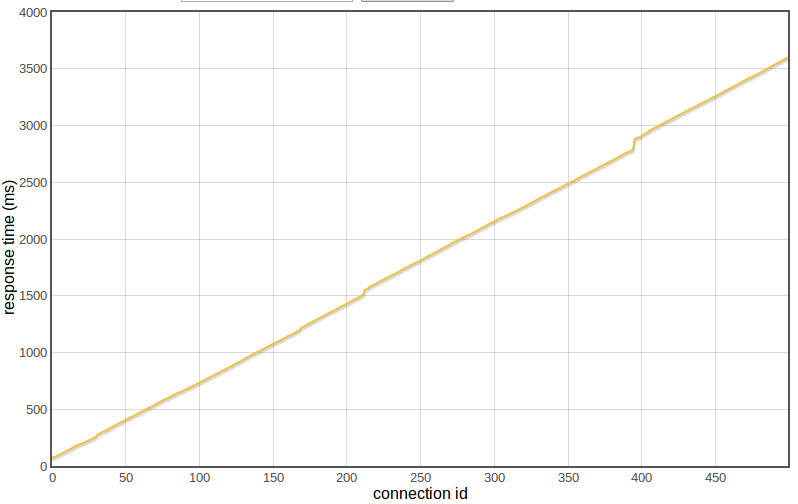
\includegraphics[scale=0.3]{performance/connection-response.png}
		% 500 gleichzeitig eingeleitete Verbindungen
		% 500 maximum des Laptops
		% maximale CPU Auslastung von etwa 15%
		% Reiner Verbindungsaufbau
		% Websocket idle bei 500 Verbindungen ist bei < 1% CPU
		% sequentielle Abarbeitung der Verbindungen
		% => Mehr User = linearer Latenzanstieg
		% 1 Thread behandelt websockets
		% => Multithreading (start simulation etc)
		%TODO Berechne durchschnittssteigerung
		%TODO Einfluss der Simulation
	
	\end{center}
\end{frame}

\begin{frame}
\frametitle{Look-Performance}
\begin{center}
	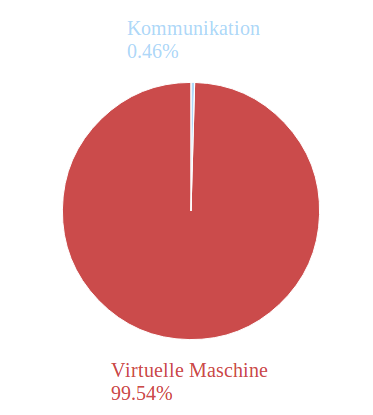
\includegraphics[scale=0.3]{performance/look-100.png}
	% 100*look
	% 80ms pro look
	% turn: 0.007824740000000002ms
\end{center}

\end{frame}

\begin{frame}
\frametitle{Move-Performance}
\begin{center}
TODO
	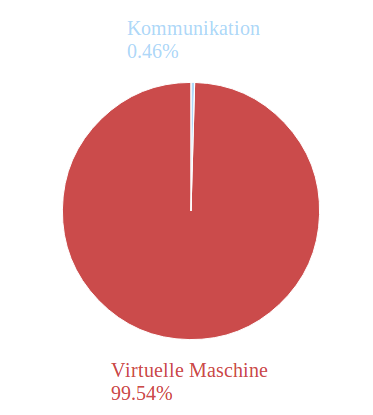
\includegraphics[scale=0.3]{performance/look-100.png}
	% 100*movement
	% turn: 0.007824740000000002ms
\end{center}

\end{frame}